\documentclass[12pt]{article}
\usepackage{tikz}
\usepackage{amsmath}
\usepackage{amssymb}
\usepackage{amsthm}
\usepackage{bm}
\usepackage{tcolorbox}
\tcbuselibrary{skins}
\usepackage{lipsum}
\usepackage[linesnumbered]{algorithm2e}
\makeatletter
\renewcommand{\@algocf@capt@plain}{above}
\makeatother
\usetikzlibrary{decorations.pathreplacing}
\usetikzlibrary{arrows}
\usetikzlibrary{snakes}
\usetikzlibrary{calc}
\let\emptyset\varnothing
\definecolor{hotpink}{rgb}{0.9,0,0.5}
\definecolor{deepgray}{gray}{0.35}
\definecolor{deepgray2}{gray}{0.25}
\definecolor{deepgray3}{gray}{0.10}
\definecolor{lightgray}{gray}{0.95}
\definecolor{lightgray2}{gray}{0.85}
\definecolor{purple1}{RGB}{239,229,244}
\definecolor{purple2}{RGB}{216,191,216}
\definecolor{lightblue}{rgb}{0.73,0.33,0.83}
\definecolor{lightpurple}{rgb}{.8,.2,.8}
\definecolor{textcolor}{rgb}{0,0,5}
\definecolor{blue1}{RGB}{187,217,238}
\definecolor{blue2}{RGB}{235,244,250}
\definecolor{yellow1}{RGB}{255,255,102}
\definecolor{blue3}{RGB}{63,40,96}
\definecolor{red1}{RGB}{255, 102, 102}
\definecolor{green1}{RGB}{102, 255, 102}
\newtheorem{lemma}{Lemma}
\newtheorem{theorem}{Theorem}
\newtheorem{definition}{Definition}
\theoremstyle{definition}
\def\proof{\par{\bf Proof}. \ignorespaces}
\def\qedsymbol{\vbox{\hrule\hbox{%
                     \vrule height1.3ex\hskip0.8ex\vrule}\hrule}}
\def\endproof{\qquad\qedsymbol\medskip\par}

% \usepackage{booktabs} % For formal tables
% \usepackage{cite}
\usepackage{url}
% \newtheorem{definition}{Definition}[section]
% \newtheorem{theorem}{Theorem}[section]
% \usepackage{algorithmic}
% \usepackage[cmex10]{amsmath}
\usepackage{amssymb}

\title{A Closer Look at Time-Preserving Walks on Evolving Graphs}

\author{Jiahao Chen and
Weijian Zhang
\thanks{%
  School of Mathematics,
The University of Manchester,
                Manchester, M13 9PL, England.
\texttt{weijian.zhang@manchester.ac.uk}.
}
}

\def\R{\mathbb{R}}
\def\C{\mathbb{C}}
\def\nbyn{n \times n}
\def\mbyn{m \times n}
\def\l{\lambda}
\def\norm#1{\|#1\|}
\def\normi#1{\|#1\|_1}
\def\normo#1{\|#1\|_{\infty}}
\def\Chat{\widehat{C}}
\def\e{eigenvalue}

% \DeclareMathOperator{\diag}{diag}   % Requires amsmath.
\def\diag{\mathop{\mathrm{diag}}}     % If not using amsmath.
\def\trace{\mathop{\mathrm{trace}}}   % If not using amsmath.

\def\At{\widetilde{A}}
\def\normt#1{\|#1\|_2}

% Note: this clashes with amsmath.
\def\bmatrix#1{\left[\matrix{#1}\right]}

\begin{document}

%\subtitlenote{The full version of the author's guide is available as
 % \texttt{acmart.pdf} document}


\maketitle

\begin{abstract}
This paper studies evolving graph centrality from the perspective of time-preserving walks. We describe time-preserving walks based on two dimensions of variation, namely static edges and causal edges.

A time-preserving walk on evolving graphs makes implicit assumptions about the type of edges that a walk traverses. For example, the walk can count only static edges or can take account of both static edges and causal edges. In addition, the length of a time-preserving walk can be either spatial or temporal.

We study the impact of different time-preserving walks on node centrality by varying the edge weights of static and causal edges.
We also compare evolving graph centrality with the aggregated static graph case to gain insight about the advantage of an evolving graph model.
We construct an evolving coauthor network from a collection of research papers for the experiments.
\end{abstract}

\section{Introduction}
\label{sec:introduction}

In the 1985 science-fiction film ``Back to the Future'', Marty McFly (played by Michael J. Fox) travelled back in time and accidentally changed history.
However, we cannot travel back in time or even send a message to the past.
To traverse an evolving graph, a.k.a a time-dependent graph, one has to consider time. In particular, a walk on an evolving graph needs to be time-preserving, meaning a node can not pass a massage (through an edge) to a node at a earlier time.

% time-respecting walk
We represent an evolving graph as a time-ordered sequences of graphs, similar to the work of Tang and coworkers \cite{nicosia13, tang09, tang102, tang10} and Grindrod, Higham and coworkers \cite{grindrod13,grindrod11}. The idea is to divide the system's time span into temporal slices and regards it as a sequence of static graphs $G^{[t]}$, one for each layer. Such representation arises naturally in many real-world applications. For example,
consider networks of users interacting through messaging. Each interaction between two users $A$ and $B$ are stored with a time stamp $t$. If we represent a user as a node then a user $A$ at time stamp $t$ is represented by a pair $(v,t)$ and a message sent from user $A$ to user $B$ at time stamp $t$ can be represented as $\langle (A, t) (B, t) \rangle$.

In general, a node $v$ on $G^{[t]}$ is represented by a pair $(v, t)$, where $t$ is the time stamp of the temporal slice.
A sequence of interactions between users form a walk. Suppose $A$ sent a message to $B$ at time stamp $t_1$
and then $B$ sent this message to $C$ at time stamp $t_2$. We can represent this activity as $\langle (A,t_1), (B,t_1), (B, t_2), (C,t_2)\rangle$, where each pair of two nodes has meanings: $\langle (A,t_1), (B,t_1) \rangle$ and $\langle (B,t_2), (C,t_2) \rangle$ represent interactions between users $A$, $B$, and $C$ and $\langle (B,t_1), (B,t_2) \rangle$ represents the fact that user $B$ holds the message at time stamp $t_1$ and $t_2$.

A time-respecting walk is a sequence of $\langle (v_1, t_1), (v_2, t_2), \ldots ,(v_m, t_m)\rangle$, where $t_1 \le t_2 \le \cdots \le t_n$ are the corresponding time stamps. If $t_i = t_j$, then $\langle (v_i, t_i), (v_j, t_j) \rangle$ is an edge where both nodes are on the same temporal slice,  otherwise it is an edge linking nodes from different temporal slices.
We call edges of the first kind \emph{static edges} and of the second kind \emph{causal edges}.
Recall in static graph, a walk of length $m$ is defined as a sequence of nodes $v_1, v_2, \ldots, v_{m+1}$ such that for each $i = 1, \ldots, m$ there is an edge from $v_i$ to $v_{i+1}$. How to determine the length of a time-respecting walk?
One could define the length of a time-respecting walk as the total number of temporal slices (see shortest temporal distance in \cite{tang09}) or the number of static edges (see dynamic walk in \cite{grindrod11}). This paper studies the impact of these two different definitions. In particular, we studies a general definition of temporal distance that takes account of both temporal slices and static edges.


% Related works
Researchers have generalised many static graph centrality algorithms for evolving graphs. One approach is to use the fact that the elements of the matrix product of adjacency matrices at different time stamps can correctly count the number of temporal walks.
However, not every centrality algorithm can be generalised in this way. Another approach is to define evolving graph centrality algorithms using time-respecting walks. This approach is applicable to algorithms that are defined using paths or walks.


% no work on pagerank so far. By understanding temporal walk, we could provide a generalization of pagerank on evolving graphs.

In Higham's following up papers, time delay is considered as alternative format of Katz centrality.
But the impact of temporal is left unconsidered. We studied the problem on centrality from two different types of centrality: one that depends on matrix unfolding and one that depends on temporal walk.


% our contribution this paper
Inspired by work
Borgatti noted in \cite{borgatti05} that the manner of traffic flow entails a new way to think about centrality.
where the author simulate different traffic flows to study centrality.

In particularly, the importance of a node in a network can not be determined without reference to how traffic flows through the network.
To develop a centrality algorithm on evolving graphs, one has to consider the manner of temporal traffic flow.
A time-preserving walk on evolving graphs can be described by static edges, causal edges, or both.



% Grindrod et al.'s definition of dynamic walk \cite{grindrod11} only counts static edges.
% Tang et al. \cite{tang10s} measure a temporal shortest walk in time unit (or causal edges) only.
% If a node can be reached by another node in $k$ time stamps then the distance between the two nodes is $k$. Chen and Zhang \cite{chen16} considered both static edges and causal edges in their definition of temporal walk.


The aims of this paper are as follows. First, to identify the type of time-preserving walk in a list of common evolving graph centrality measures. Second, to vary static and causal edge weights and analyze the impact on selected measures of centrality.
Third, to solve a real world problem using evolving graph centrality: identify key authors in an evolving coauthor network.
We carry out the experiment using the Julia dynamic network analysis package
EvolvingGraphs.jl (\url{https://github.com/EtymoIO/EvolvingGraphs.jl}).
We use the research paper data gathered from Etymo (\url{https://etymo.io}), a visual search engine for data scientists.



\section{Time-Preserving walks}
\label{sec:time-pres-walks}

For example, in Figure \ref{fig:eg_shortest_walk}
$\langle (1, t_1), (2, t_1) \rangle$ is a static edge at time stamp $t_1$ and $\langle (3, t_2), (3, t_3) \rangle$ is a causal edge between time stamp $t_2$ and time stamp $t_3$.
The difference between static edges and causal edges were first explicitly considered in \cite{chen16}.

\begin{figure}[h]
 \begin{center}
    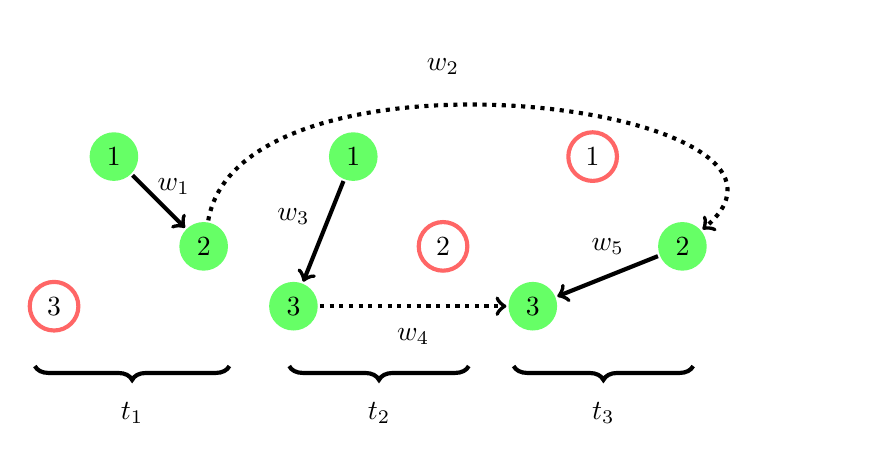
\begin{tikzpicture}[scale=.38, line width =1.5pt]
  \node[circle,fill=green1, minimum size=0.2cm] (n7) at (-5,7) {2};
  \node[circle,draw=red1, minimum size=0.2cm] (n8) at (-10,5) {3};
  \node[circle,fill=green1, minimum size=0.2cm] (n10) at (-8,10) {1};
  \node[circle,draw=red1, minimum size=0.2cm] (n6) at (3,7) {2};
  \node[circle,fill=green1, minimum size=0.2cm] (n4) at (-2,5) {3};
  \node[circle,fill=green1, minimum size=0.2cm] (n1) at (0,10) {1};
   \node[circle,fill=green1, minimum size=0.2cm] (n11) at (11,7) {2};
  \node[circle,fill=green1, minimum size=0.2cm] (n12) at (6,5)  {3};
  \node[circle,draw=red1, minimum size=0.2cm] (n14) at (8,10) {1};
  \node (w1) at (-6, 9) {$w_1$};
  \node (w2) at (3, 13) {$w_2$};
  \node (w3) at (-2, 8) {$w_3$};
  \node (w4) at (2, 4) {$w_4$};
  \node (w5) at (8.5, 7) {$w_5$};s
  \foreach \from/\to in {n10/n7, n1/n4, n11/n12}
   \draw[every edge,->] (\from) -- (\to);
 \draw[dotted,->](n4) -- (n12);
\draw[dotted,->](n7) to[out=80, in=40](n11);
\draw [decorate,decoration={brace,amplitude=5pt},xshift=-4pt,yshift=0pt]
(4,3) -- (-2,3) node [midway,yshift=-0.6cm]{ $t_2$};
\draw [decorate,decoration={brace,amplitude=5pt},xshift=-4pt,yshift=0pt]
(-4,3) -- (-10.5,3) node [midway,yshift=-0.6cm]{ $t_1$};
\draw [decorate,decoration={brace,amplitude=5pt},xshift=-4pt,yshift=0pt]
(11.5,3) -- (5.5,3) node [midway,yshift=-0.6cm]{ $t_3$};
    \end{tikzpicture}
\end{center}
\caption{An evolving directed graph with 3 time stamps $t_1$, $t_2$ and $t_3$.
At each time stamp, the evolving graph is represented as a graph.
The green filled circles represent active nodes while the red circles represent
inactive nodes. Directed edges in each time stamp are shown as black arrows and directed edges between graphs are shown as dotted arrows, where $w_1, w_2 \ldots w_5$ are edge weights.}
\label{fig:eg_shortest_walk}
\end{figure}

It is natural to define the length of a walk on a static graph as the number of nodes travelled through the walk. For the weighted graph case, the length of a walk is the total weight of all the edges in the walk. We observe that static edges link nodes in space while causal edges link nodes in time. Hence we would like to distinguish temporal distance from spatial distance on an evolving graph: the length of a static edge is equal to the edge weight (or $1$ in the unweighted graph case); the length of a causal edge is the time distance between the two nodes. In the simplest case, the time-respecting walk
$\langle (1, t_1) ,(2, t_1) , (2, t_3), (3, t_3)\rangle$ in Figure \ref{fig:eg_shortest_walk} has length $4$ in total because two static edges $\langle (1, t_1) (2, t_1) \rangle$ and $\langle (2, t_3), (3, t_3) \rangle$ have length one, whereas $\langle (2, t_1) (2, t_3) \rangle$ traverse $2$ time stamps so has length $2$.

We now describe time-preserving walks in more detail. We follow the definition of
\emph{evolving graph}, \emph{temporal node} and \emph{active node} in \cite{chen16}.

\begin{definition}
  An \textbf{evolving graph} $G_n$ is a sequence of (static) graphs
$G_n = \langle G^{[1]}, G^{[2]},  \ldots ,G^{[n]} \rangle$ with associated time stamps
$t_1, t_2, \ldots, t_n$ respectively. Each $G^{[t]} = (V^{[t]}, E^{[t]})$ represents a (static) graph labeled by a time t.
\end{definition}

Note the node sets $V^{[t]}$ can change over time, i.e., nodes may appear or disappear at a particular time stamp.
For example, in Figure \ref{fig:eg_shortest_walk}, at time stamp $t_1$, $V^{[1]} = \langle 1, 2 \rangle$ and $E^{[1]} = \langle (1,2) \rangle$. Each graph $G^{[t]}$ can be represented by its adjacency matrix $A^{[t]}$.
We can represent $G_n$ by a list of adjacency matrices $A_n = \langle A^{[1]}, A^{[2]}, \ldots, A^{[n]} \rangle$.


\begin{definition}
  A \textbf{temporal node} is a pair (v, t), where $v \in V^{[t]}$ is a node at a time $t$.
\end{definition}

%At each time stamp, we only count temporal nodes that connects by an edge.

\begin{definition}
  A temporal node $(v, t)$ is an \textbf{active node} if there exists at least one edge $e \in E^{[t]}$ that connects $v \in V^{[t]}$ to another node $w \in V^{[t]}, w\ne v$. Otherwise it is called an inactive node.
\end{definition}

In Figure \ref{fig:eg_shortest_walk}, the filled green circles are active nodes. For the adjacency matrix representation, a node $i$ is active at time stamp $t$, then
the $i$th row or the $i$th column of $A^{[t]}$ has at least one none-zero entry.
 In general, a time-preserving walk can be defined as follows.

\begin{definition}
A \textbf{time-preserving walk}  of length $m$ on an evolving graph $G_n$ is a time-ordered sequence of active nodes, $\langle (v_1, t_1), (v_2, t_2), \ldots, (v_m, t_m) \rangle$, where $t_1 \le t_2 \le \cdots \le t_m$ and
$v_i = v_j$ if and only if $t_i \ne t_j$.
\end{definition}

Note $\langle (v_i, t_i), (v_j, t_i) \rangle$ represents a static edge on graph $G^{[t_i]}$ while $\langle (v_i, t_i), (v_i, t_j) \rangle$ represents a causal edge from time stamp $t_i$ to time stamp $t_j$.

\begin{definition}
A \textbf{static edge} $\langle (v_i, t), (v_j, t)\rangle$ is a pair of elements of $V^{[t]}$, i.e., $v_i \in V^{[t]}$ and
$v_j \in V^{[t]}$.
 A \textbf{causal edge} $\langle (v, t_i), (v, t_j)\rangle$ is a pair of the same node at different time stamps.
\end{definition}

We can denote a \emph{weighted static edge} as $\langle (v_i, t), (v_j, t), w_s \rangle$ and a \emph{weighted causal edge} as $\langle (v, t_i), (v, t_j), w_t \rangle$.
Here $w_s$ represents the spatial distance between the two nodes $v_i$ and $v_j$; $w_t$ represents the
temporal distance of $v$ at different time stamps.
In Figure \ref{fig:eg_shortest_walk}, the black arrows represent static edges and the dotted arrows represent causal edges.
Suppose we assign all the static edge weight to be $1$ and
assign the causal edge to be the number of time stamps between the pair. Then in Figure \ref{fig:eg_shortest_walk}
the edge weight between $(1, t_1)$ and $(2, t_1)$ is $1$ and the edge weight between $(2, t_1)$ and $(2, t_3)$
 is $2$.

A time-preserving walk can traverse both causal edges and static edges.
We will see in the next section that evolving centrality measures make implicit assumptions about the type of edges in the
time-preserving walk that is used.



\section{Centrality Measures}
\label{sec:topol-temp-flow}

In \cite{tang10s}, a temporal shortest walk is measured in time units only, i.e., if node
$v_i$ can reach node $v_j$ in $k$ time steps then the distance between node
$v_i$ and $v_j$ is $k$. We can apply temporal breadth first
search (BFS) \cite{chen16} to discover the temporal walks and then only take account of the temporal difference between the first node $(v_1, t_1)$ and the last node $(v_n, t_n)$, i.e., $t_n - t_1$.

If we use this definition of temporal walk for the temporal Katz centrality introduced in
\cite{grindrod11}, we have a new centrality measure.
In the matrix form, the nonzero entries of $A^{[t_i]} A^{[t_{i+1}]}$ counts all the temporal walks of length $1$, and
$A^{[t_i]}\cdots A^{[t_j]}$, where $i < j$ counts all the temporal walks of length $j -i$.
For example, $A^{[1]}A^{[4]}$, $A^{[1]}A^{[1]}A^{[4]}$ and $A^{[1]}A^{[2]}A^{[3]}A^{[4]}$ are all walks of length 3.
In the original Katz centrality, the `attenuation' factor $\alpha$ is imposed on the
number of walks, i.e., longer walks has smaller effect to the overall rating.
Hence the final result is the summation of all products of the form
\[
\alpha^k A^{[i]} \cdots A^{[i+k]}
\]
% Note this can not be written in \eqref{eq:katz}, as discussed in Section \ref{sec:temp-katz-centr}.


Another definition of temporal walk was introduced by \cite{chen16}. Here
both static edges and causal edges are considered. We can represent an evolving graph by a block adjacency matrix, as shown in Section \ref{sec:centr-block-adjac}. Centrality on this block matrix gives the importance of each node at all time stamps. We can average these rating at different time stamps to
get the final rating.


We review a few well-known measures of evolving graph centrality.
(Design a simple example and discuss it in each case below.)


\subsection{Temporal Katz Centrality and Communicability Betweenness Centrality}
\label{sec:temp-katz-centr}

The Katz Centrality is a measure of importance

In \cite{grindrod11}, Grindrod et al. define a \emph{dynamic walk} of length $m$ from
node $v_1$ to node $v_{w+1}$  as a sequence of edges
$(v_1, v_2), (v_2, v_3), \ldots (v_w, v_{w+1})$ and a non-decreasing sequence of times
$t_{r_1} \leq t_{r_2} \leq \cdots \leq t_{r_w}$ such that the adjacency matrix at time stamp
$r_m$, i.e., $A_{i_m, i_{m+1}}^{[r_m]} \ne 0$. Note that in this definition the authors only take account of the static edges and the length of a dynamic walk is determined by the number of static edges.

The Katz centrality is based on a sequence of matrix products
\begin{equation}
\label{eq:katz}
Q = (I - \alpha A^{[0]})^{-1}(I - \alpha A^{[1]})^{-1} \cdots (I - \alpha A^{[M]})^{-1}.
\end{equation}
The $i$th row and column sums
$$
C_i^{broadcast} = \sum_{k=1}^n Q_{ik}, \quad C_i^{receive} = \sum_{k=1}^n Q_{ki}
$$
are the broadcast centrality and receive centrality of node $i$.

\subsection{Temporal Betweenness and Closeness Centrality}
\label{sec:temp-betw-centr}

Recall that betweenness centrality of a node in a static graph is defined by counting the fraction of shortest walks that traverse it.
We could extend
betweenness centrality on evolving graphs by replacing shortest walks with temporal shortest walks \cite{nicosia13}.
\begin{equation}
  \label{eq:bet1}
C_i^{betweenness} = \sum_{j \in V}\sum_{k \in V, k \ne j}\frac{\alpha_{jk}(i)}{\alpha_{jk}},
\end{equation}
where $\alpha_{jk}$ represents the number of temporal shortest walks from node $j$ to node $k$ and $\alpha_{jk}(i)$ represents the number of temporal shortest walks from node $j$ to node $k$ that pass through the node $i$.

One may want to take into account the length of time a node passes a message. The temporal betweenness centrality of the node $i$ at time stamp $t_m$ is defined as
\begin{equation}
  \label{eq:bet2}
  C_i^{betweenness}(t_m) = \sum_{j\ne i}\sum_{k\ne j, k\ne i}\frac{U_{j,k,t_m}(i)}{\alpha_{j,k}},
\end{equation}
where, as before, $\alpha_{j,k}$ represents the number of temporal shortest walks from $j$ to $k$ and $U_{j,k,t_m}(i)$ represents the number of temporal shortest walks from $j$ to $k$ in which node $i$ is traversed from
the walk in the time stamp $t_m$ or a previous time stamp $t_{m-1}$. Then
average temporal betweenness of node $i$ is then defined as
$$
  C_i^{betweenness} = \frac{1}{M}\sum_m C_i^{betweenness}(t_m).
$$
Note \eqref{eq:bet1} only takes account of static edges while \eqref{eq:bet2} takes account of both static edges and causal edges.

% closeness centrality
Similar to betweenness centrality, let $d_{ij}$ be the length of a temporal shortest walk from $i$ and $j$ in an evolving graph. Then
the closeness centrality of a node $i$ is defined
$$
C_i^{closeness} = \frac{N-1}{\sum_j d_{ij}}.
$$
Note that this depends on how we define the length of temporal shortest walk. The closeness centrality can takes account of only static edges, only causal edges, or both.


\subsection{Mapping from Evolving Graphs to Static Graphs}
\label{sec:centr-block-adjac}

In \cite{chen16}, we derive a block adjacency matrix representation of an evolvign graph.
If $E'$ is the set of causal edges and $\hat E$ is the set of static edges then
an evolving graph can be represented as
$$
\bm M_n =
\begin{pmatrix}
A^{[t_1]} & M^{[t_1, t_2]} & \ldots & M^{[t_1, t_n]} \\
0         & A^{[t_2]} & \ldots & M^{[t_2, t_n]} \\
          & \ldots    &        &     \\
0         & 0         & \ldots & A^{[t_n]}
\end{pmatrix},
$$
where $M^{[t_i, t_j]}$ is the matrix whose rows are labeled by $V^{[t_i]}$ and columns are labeled by $V^{[t_j]}$, and whose entries are
$$
  M_{uv}^{[t_i, t_j]} =
  \begin{cases}
    1 & \mbox{if} (u, v) \in E' \\
    0 & \mbox{otherwise}.
  \end{cases}
$$
The adjacency matrix blocks $A^{[t]}$ encode the static edge set $\hat E$, whereas the off-diagonal blocks $M^{[t_i, t_j]}$ encode the causal edge set $E'$.

(Need to justify the benefit of this approach.)
We can apply static graph centrality algorithms to $M_n$ and then take the average of ratings at each each time stamp. For example, we can construct the Google matrix
$G_n$ from $M_n$ and the ranking of the nodes can be found by solving
$$
 r= G_n r.
$$

For Figue \ref{fig:eg_shortest_walk}, we have

\begin{align*}
V & = \{(1,\!t_1), (2,\!t_1), (1,\!t_2), (3,\!t_2), (2,\!t_3), (3,\!t_3)\},\\
\tilde E &= \{((1,\!t_1), (2,\!t_1)), ((1,\!t_2), (3,\!t_2)), ((2,\!t_3), (3,\!t_3))\},\\
E'  &= \{((1,\!t_1), (1,\!t_2)), ((2,\!t_2), (2,\!t_3)), ((3,\!t_2), (3,\!t_3))\}.
\end{align*}

and corresponding block adjacency matrix is

\[
\bm M_3 = \begin{pmatrix}
0 & 1 & 1 & 0 & 0 & 0 \\
0 & 0 & 0 & 0 & 1 & 0 \\
0 & 0 & 0 & 1 & 0 & 0 \\
0 & 0 & 0 & 0 & 0 & 1 \\
0 & 0 & 0 & 0 & 0 & 1 \\
0 & 0 & 0 & 0 & 0 & 0
\end{pmatrix}
\]

The static graph representation of Figure \ref{fig:eg_shortest_walk} is shown in Figure \ref{fig:static}.

\begin{figure}[h]
 \begin{center}
   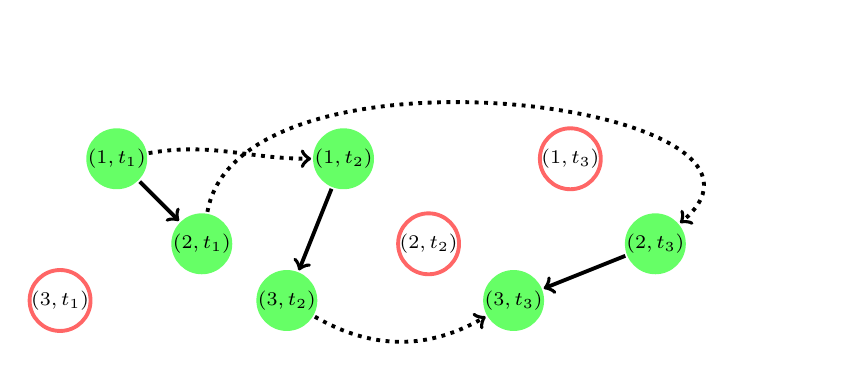
\begin{tikzpicture}[scale=.36, line width =1.4pt]
  \node[circle,fill=green1, minimum size=0.1cm, inner sep = 0pt] (n7) at (-5,7)
{\scriptsize $(2,t_1)$};
  \node[circle,draw=red1, minimum size=0.2cm, inner sep = 0pt] (n8) at (-10,5)
{\scriptsize $(3,t_1)$};
  \node[circle,fill=green1, minimum size=0.1cm, inner sep = 0pt] (n10) at (-8,10) {\scriptsize $(1,t_1)$};

  \node[circle,draw=red1, minimum size=0.2cm, inner sep = 0pt] (n6) at (3,7)
{\scriptsize $(2,t_2)$};
  \node[circle,fill=green1, minimum size=0.2cm,  inner sep = 0pt] (n4) at (-2,5)
{\scriptsize $(3,t_2)$};
  \node[circle,fill=green1, minimum size=0.2cm,  inner sep = 0pt] (n1) at (0,10)
{\scriptsize $(1,t_2)$};

   \node[circle,fill=green1, minimum size=0.2cm,  inner sep = 0pt] (n11) at (11,7)
{\scriptsize $(2,t_3)$};
  \node[circle,fill=green1, minimum size=0.2cm,  inner sep = 0pt] (n12) at (6,5)
{\scriptsize $(3,t_3)$};
  \node[circle,draw=red1, minimum size=0.2cm,  inner sep = 0pt] (n14) at (8,10)
{\scriptsize $(1,t_3)$};

  \foreach \from/\to in {n10/n7, n1/n4, n11/n12}
   \draw[every edge,->] (\from) -- (\to);
     \draw[dotted,->](n7) to[out=80, in=40] (n11);
  \draw[dotted,->](n10) to[out=10, in=180] (n1);
   \draw[dotted,->](n4) to[out=-30,in=-150] (n12);
    \end{tikzpicture}
\end{center}
\caption{A static graph corresponding to the evolving graph example of
Figure~\ref{fig:eg_shortest_walk}. The green nodes are active nodes while the
red nodes are inactive nodes.
The black lines are edges in the static edge set $\tilde E$ and are encoded
algebraically in the diagonal blocks $A^{[t]}$ of the adjacency matrix $\bm M_3$.
The dotted lines are edges in the causal edge set $E'$ and are encoded algebraically in
the off-diagonal blocks $M^{[t_i, t_j]}$.
The graph containing all the edges and temporal nodes has adjacency matrix $\bm M_3$.}
\label{fig:static}
\end{figure}


\subsection{Reverse Temporal Flows}
\label{sec:reverse-temp-flows}

We can not travel back in time. But reversing the direction of temporal flows can help
identify the ``hub'' nodes or the source of the flows. The authority score of a page is
proportional to its importance, and the hub score describes the quality of a page as a link collection of important related pages \cite{kleinberg99}.
Indeed, reverse PageRank has
been studied by \cite{bar08, fogaras03, gleich15}. In reverse PageRank we compute PageRank on the graph with reversed direction, i.e., reverse the direction of each edge $(i,j)$ to $(j, i)$.
Fogaras \cite{fogaras03} shows that Reversed Page Rank scores express hub quality.


Recall a time-preserving walk is a time-ordered sequence of active nodes. Here we define a \emph{reversed temporal walk} to be a reversed time-ordered sequence of active nodes, i.e.,
$t_1 \ge t_2 \ge \cdots \ge t_m$.

\subsection{Temporal PageRank}

We consider two generalisation of pagerank: a block matrix one and a dense matrix one that is based on probability


\section{Experiments}
\label{sec:experiments}

In this section, we vary the edge
weights in both static and causal edges to study the impact of time-preserving walks on evolving graph centrality.
We also compare evolving graph centrality with the aggregated static graph case to gain insight about the advantage of evolving graph model.

\subsection{JMLR Coauthor Network}
\label{sec:jmlr-coauth-netw}


We construct the evolving coauthor network from Etymo (\url{https://etymo.io}).
We collected $1566$ publications published by Journal of Machine Learning Research (JMLR) from $2001$ to $2017$ with authors involved. We regard each year
as a time stamp and there are $17$ time stamps in total. At each time stamp, we
create a undirected edge (or two directed edges) between two authors if they have coauthored at least one paper.
(add results here.)

A second network is constructed by linking leading authors in different papers whose
ideas are similar. The resulting network represent the connectivity of ideas in all the research papers in the database.

(add results here.)

\subsection{Paper Keyword Tag Network}

We tag our research articles by subjects.

We can construct a time-dependent tag network by link tags in each articles. For example,
suppose a paper $p_1$ has three tags $t_1$, $t_2$, and $t_3$, where $t_1$ is a superclass of $t_2$ and $t_3$.
We link $t_2$ and $t_3$ in both direction and create a link from $t_1$ to $t_2$ and a link from $t_1$ to $t_3$.
The time stamp of these edges is the published date of the paper.



\section{Conclusion}
\label{sec:conclusion}

To write later.

\bibliographystyle{plain}
\bibliography{sigproc}

\end{document}

%%% Local Variables:
%%% mode: latex
%%% TeX-master: t
%%% End:
